\documentclass{llncs}
\usepackage[utf8]{inputenc}
\usepackage[russian]{babel}
\usepackage[pdftex]{graphicx}
\usepackage{comment}
\usepackage{cite}
\usepackage{cmap}
\usepackage{setspace}
\usepackage{authblk}
\usepackage{amsmath}
\usepackage{amssymb}
\usepackage{siunitx}

\graphicspath{{pic/}}
\DeclareGraphicsExtensions{.eps,.pdf,.png,.jpg}

\usepackage{tabularx}
\usepackage{multicol}
\usepackage{epstopdf}

\usepackage{subfig}
\usepackage[font={footnotesize,sl}]{caption}

% Номера страниц сверху и по центру
%\def\headfont{\small}
%\pagestyle{headcenter}
%\chapterpagestyle{empty}

\pagestyle{plain}

% Использовать полужирное начертание для векторов
\let\vec=\mathbf

% Включать подсекции в оглавление
\setcounter{tocdepth}{2}

\usepackage{indentfirst}

\usepackage{bm}
\usepackage{empheq}
\usepackage{longtable}
\usepackage{multirow}
\usepackage{multicol}
\usepackage{tikz}
\usetikzlibrary{shapes,shapes.geometric,arrows,fit,calc,positioning,automata}
\usetikzlibrary{arrows.meta}
\usetikzlibrary{shapes.multipart}
\usetikzlibrary{patterns}
\usetikzlibrary{decorations.pathreplacing}

\usepackage{extarrows}
\usepackage{rmathbr}
\usepackage{embrac}
\usepackage{todonotes}


\title{Реализация эффекта захвата канала в программно-конфигурируемом радио}
\author{
Глинский К., Куреев А.\\
\{kglinsk\}@yandex.ru, \{kureev\}@iitp.ru\\
}
\institute{ИППИ РАН}

\begin {document}
\maketitle

\begin{abstract}
В сетях стандарта 802.11 при одновременной передаче нескольких участников на одной частоте возможно пересечение нескольких кадров. Согласно действующему стандарту приемник должен просигнализировать о коллизии и не принять ни один из кадров. Тем не менее, если существенно более слабый сигнал поступил раньше, то существует  возможность произвести пересинхронизацию и принять более сильный сигнал при достаточном соотношении мощностей. Данный эффект называется эффектом захвата канала, и способен влиять на ключевые параметры параметры сети. В данной работе для экспериментального изучения эффекта используется  программно-конфигурируемое радио NI USRP 2944 RIO, на котором в рамках  исследования  был имплементирован эффект захвата канала.
\end{abstract}

\keywords{Эффект захвата канала, USRP, скрытые станции, IEEE 802.11 }

\section{Введение}
В настоящее время технология беспроводных сетей стандарта 802.11 широко распространена$^{[1]}$, и прогнозируется дальнейший рост как количества подключенных устройств, так и обьемов передаваемых по сети данных. Таким образом, актуальными становятся исследования механизмов, позволяющих повысить пропускную способность и снизить задержки в условиях плотных сетей и высоких показателей загрузки каналов сети, а также снизить влияние соседствующих и интерферирующих станций. Одним из таким механизмов является эффект захвата канала, который способен существенно повысить пропускную способность сети в некоторых сценариях использования сети$^{[2]}$. Данный эффект заключается в возможности декодировать более сильный сигнал при пересечении кадров при передаче в одном диапазоне частот.Эффект захвата канала изучен методами математического моделирования при различных предположениях о параметрах сети$^{[3]}$. Проводилось и имитационное моделирование данного эффекта. Тем не менее, проведенные  экспериментальное исследования требовали либо сложной архитектуры и методологии проведения эксперимента$^{[4]}$, либо могли проводиться на основе off-the-shelf сетевых устройств с изменением работы  только на уровне драйверов оборудования$^{5}$. Известен также патент$^{[6]}$ на устройство, использующее эффект захвата канала в беспроводных сетях, работающих по методу доступа CSMA/CA. Новизна данной статьи состоит в том, что устройство с эффектом захвата реализовано на программно-конфигурируемом оборудовании, что позволяет осуществлять гибкую настройку параметров приемника.
\section{Эффект захвата канала в сетях 802.11}
Стандарты 802.11 определяют структуру кадра и распределение ресурсов между участниками сети. В качестве алгоритма случайного доступа используется метод CSMA/CA, регламентирующий  доступ к каналу и механизм разрешения коллизий. В отсутстие эффекта захвата, оба пакета будут считаться недействительными. Однако, если эффект захвата канала реализован, то возможно принять более сильный кадр, если разница мощностей между ними $\Delta$W$_{RX}$ превосходит необходимое для используемой сигнально-кодовой конструкции соотношение сигнал-шум. В таком случае можно выделить два варианта. 
\begin{enumerate}
\item Более мощный пакет приходит первым, успешно проходит синхронизация и прием данных, слабый же пакет теряется. Данный вариант изображен на рис. 1\\

\begin{figure}[]
\center{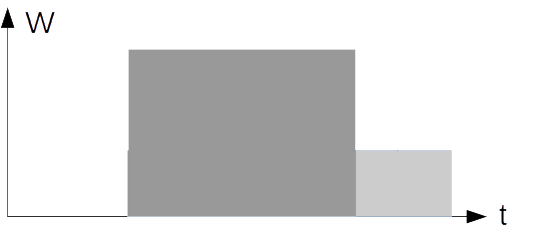
\includegraphics[scale=0.5]{capture_effect_init.png}}
\caption{Сценарий приема 1}
\label{ris:image}
\end{figure}

\item Более мощный пакет приходит вторым, и приемник уже синхронизировался на первый слабый пакет. В таком случае второй пришедший пакет приводит к потере обоих пакетов в отстутствие эффекта, и приему сильного в случае пересинхронизации на него. Отметим, что в зависимости от соотношений  длин кадров, возможно две ситуации. Обозначим время передачи сильного и слабого кадров как t$_{high}$ и t$_{low}$ соответственно, а смещение одного кадра относительно другого за $\Delta$t. Разность мощностей на входе для слабого и сильного кадра обозначим как $\Delta$W, равная W$_{RX high}$ - W$_{RX low}$. В таком случае возрастание мощности $\Delta$W$_{rise}$  равна $\Delta$W , а величина падения мощности при завершении приема сильного кадра составит $\Delta$W$_{drop}$ = $\Delta$W в случае 2.1 и W$_{RX high}$ в случае 2.2.
\\
\begin{figure}[]
\center{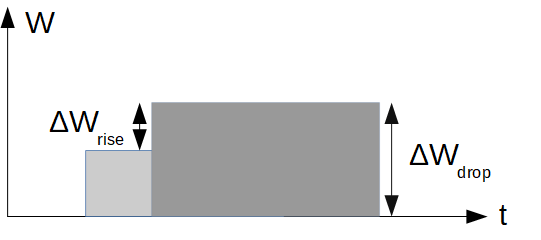
\includegraphics[scale=0.5]{capture_effect_scenario_1.png}}
\caption{Сценарий приема 2.1, t$_{low}$ < t$_{high}$+$\Delta$t}
\label{ris:image}
\end{figure}
\begin{figure}[]
\center{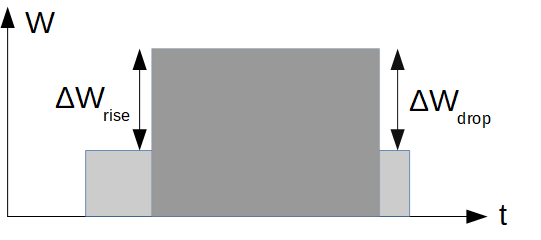
\includegraphics[scale=0.5]{capture_effect_scenario_2.png}}
\caption{Сценарий приема 2.2, t$_{low}$ > t$_{high}$+$\Delta$t}
\label{ris:image}
\end{figure}

\end{enumerate}
Данный эффект способен оказывать как положительное влияние на пропускную способность сети в сценариях с многочисленными скрытыми станциями и плотной сетью подключений,что было проверено в исследовании$^{[5]}$, так и потенциально нарушать справедливость механизма распределения ресурсов между участниками сети, предоставляя наиболее мощному источнику преимущество при приеме.  

\section{Имплементация алгоритма в USRP}
\subsection{Формулировка требований к алгоритму}
К алгоритму, реализованному в USRP для наблюдения эффекта захвата канала,  предьявляются следующие требования
\begin{enumerate}
\item Обладать  обратной совместимостью с оборудованием не поддерживающим данный эффект, и соответствовать основным требованиям различных редакций стандарта 802.11
\item Иметь возможность регулировать предельные параметры  сигналов, при которых  начинает происходить пересинхронизация приемника. 
\item Обеспечивать корректное начало приема более сильного сигнала вместе с освобождением всех данных слабого пакета из памяти и буферов обмена, разделяя обработку данных принятых из двух пакетов вне зависимости от сдвига по времени двух пакетов между собой.
\item Минимизировать количество ложных срабатываний эффекта при различных сценариях 
использования устройства.
 
\end{enumerate}  В качестве
основного признака, на основании которого можно предполагать коллизию двух пакетов с различными параметрами, было выбрано изменение значение мощности входящего сигнала во время приема пакета на величину выше определенного порога. Данный признак был выбран в силу следующих предположений \begin{enumerate}
\item Мощность сигнала от одной станции слабо меняется в течении передачи одного кадра. 
\item Характеристики канала также не изменяются за время порядка одного пакета. 
\item Детектирование эффекта должно быть произведено и обработано за минимально возможное время.

\end{enumerate} 
Условие срабатывания эффекта по превышению порога мощности удовлетворяет поставленным условиям,так как вычисление мощности входного радиосигнала выполняется за 64 отсчета АЦП с частотой 80 MSPS , а изменение мощности приемника за  время передачи кадра предполагается малым.
\\\
\subsection{Алгоритм реализованного эффекта}
После обнаружения скачка входной мощности логическая защелка устанавливается в новое состояние, не допуская дальнейшие избыточные попытки пересинхронизации до прихода сигнала сброса защелки. Сигналом сброса выступает падение входной мощности на величину выше порога, сигнализирующая о завершении кадра и готовности к принятию следующих. Данный алгоритм отличается от предлагаемого в патенте$^{[6]}$, в котором при наложении двух кадров возможно несколько пересинхронизаций из=за дискретности и задержек отсчета мощности, что может привести к невозможности принять кадр.
\\
После срабатывания данного эффекта происходит переключение машины состояний, реализованной внутри FPGA USRP в состояние поиска синхронизации (детектирование преамбулы ). Одновременно происходит перенастройка модуля CFO (Central frequency offset), устанавливающий величину сдвига частоты относительнно эталонной. 
\\
На следующем этапе происходит обработка IQ, состоящая из преобразования Фурье, который сбрасывается в исходное состояние на время от детектирования подъема мощности до сигнала о начале пакета, оценки канала и коррекции фазы ( перерасчитываемой при подъеме мощности) и выделении пилотных поднесущих сигнала.
\\
В дальнейшем поднесущие поступают в модуль обработки битов, состоящий из  сериализатора битов, демаппера, декодера Витерби, которые приводятся к исходному состоянию. Также сбрасываются  очереди данных и счетчики на все время действия защелки 1. Помимо этого все биты пришедшие во время защелки, обозначаются как не валидные и не передаются на дальнейшую обработку. Еще одна очистка происходит на этапе перевода массива битов в байты PSDU, при которой биты и индекс записываемого  бита в массиве  перезаписываются нулями.
\\
Изменения были внесены и в машину состояний, отвечающую за управление приемом пакетов. Добавленные функции позволяют переключиться в режим окончания приема и корректно его завершить из любого исходного состояния машины. 
\\
Модули, обрабатывающие пакеты на MAC уровне также были переработаны. Был реализован сброс дизассемблера пакета, расчета контрольной суммы, а также машины состояний MAC уровня.
\\
Вышеописанные изменения позволяют  обработать и принять данные более сильного пакета до завершения приема и сигнала о принятии последнего сэмпла, после чего происходит сброс защелки (вследствие падения мощности радиосигнала) и станция становится готова к приему следующего пакета.
\\
Схема реализованного алгоритма представлена на рис. 4
\begin{figure}[htp!]
\center{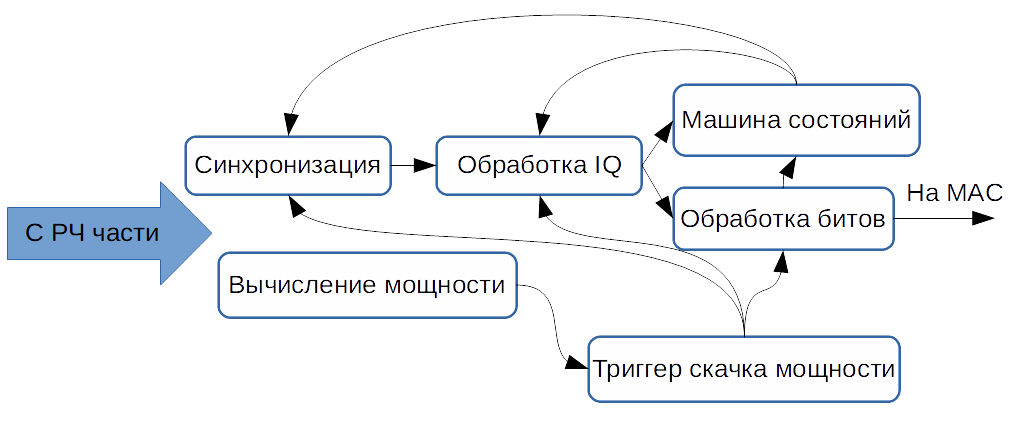
\includegraphics[scale=0.5]{scheme.png}}
\caption{Блок-схема PHY уровня установки}
\label{ris:image}
\end{figure}


\section{Экспериментальная проверка эффекта}
Для экспериментальной проверки работоспособности устаноки использовался сценарий эффекта захвата с двумя станциями-передатчиками, отправляющими пакеты с заданными разностью мощностей сигналов и сдвигом по времени (меньше длины пакета). Схема данного эксперимента приведена на рисунке ниже. 
\\
При проверке работоспособности реализованного эффекта захвата канала были произведены 2 эксперимента 
\begin{enumerate}
\item Замер FRR (отношение принятых пакетов к количеству отправленных) в зависимости от временного сдвича между двумя пакетами, где длина пакета составила 1000 байт, а время передачи кадра -1430 мкс при СКК 0. 
\item Замер FRR для различных СКК и варьируемой разности мощности между пакетами.
\end{enumerate}
\begin{figure}[ht!]
\center{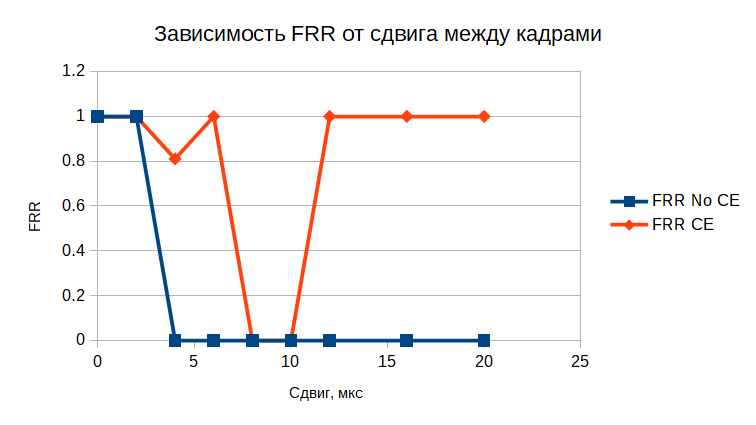
\includegraphics[scale=0.5]{frr_0.png}}
\center{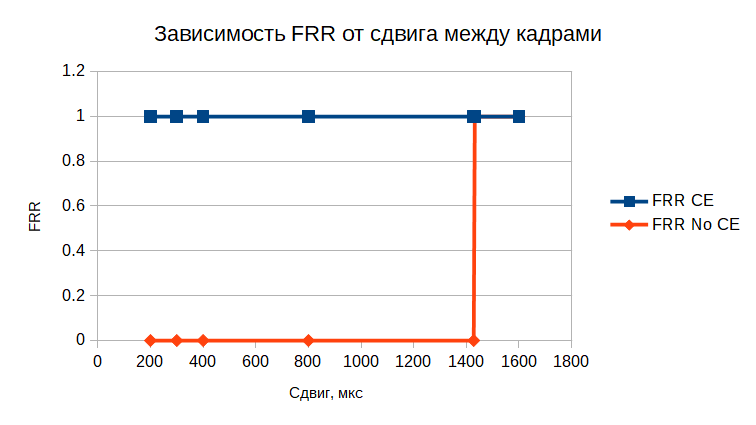
\includegraphics[scale=0.5]{frr_200.png}}

\caption{Зависимость FRR от сдвига между пакетами.}
\label{ris:image}
\end{figure}
Приложенный график демонстрирует, что данная установка позволяет обеспечить близкий к 1 FRR для второго пакета при пересечении пакетов на более чем 12 мкс, то есть после синхронизации на первый пакет, в отличие от стандартного режима работы, при котором FRR равен 0. Отметим, что при  смещении кадров на 4 мкс FRR обращается в 0 для стандартного режима вследствие того, что приемник успевает начать синхронизоваться на первый кадр, что приводит к некорректному приему. Для реализованной установки второй кадр не принимается только при сдвиге от 6 до 12 мкс, что связано с проведенной не до конца синхронизацией на первый кадр, за счет чего пересинхронизация не срабатывает.%%Реализация устойчивой работы пересинхронизации при любой задержке представляет собой одну из перспектив дальнейших исследований
\\
\begin{figure}[htp!]
\center{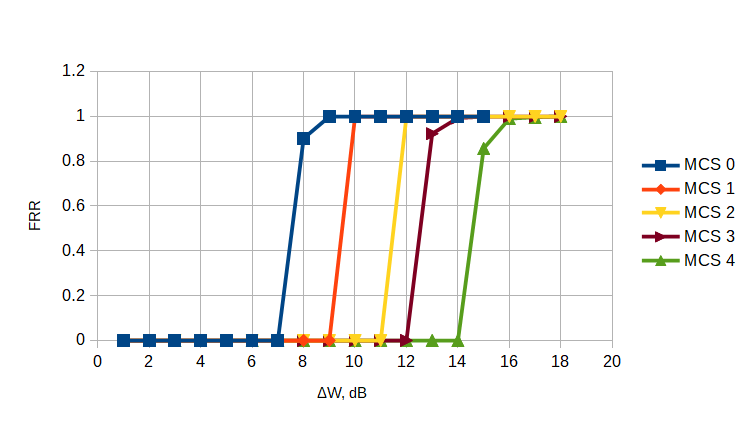
\includegraphics[scale=0.5]{MCS_difference.png}}
\caption{Зависимость FRR от соотношения $\Delta$W$_{RX}.$}
\label{ris:image}
\end{figure}
График на рис.6 показывает связь между FRR и разности мощностей между пакетами для различных СКК при фиксированном пороге детектирования второго пакета, равному $\Delta$W$_{detect}$=8 dB. Видно, что с  увеличением номера СКК необходимая для корректного приема разность мощностей возрастает. Поскольку после пересинхронизации первый кадр продолжает передаваться, то соотношение сигнал/шум в канале определяется разностью мощности двух кадров $\Delta$W$_{RX}$. Таким образом, на возможность принятия кадра влияет как порог детектирования второго кадра, равный 8 дБ в эксперименте, так и минимальное значение SNR для СКК. Из графика видно, что при СКК выше второго определяющую роль играет значение SNR.
\section{Заключение}
Сети стандарта 802.11 стандарта 802.11 подвержены влиянию эффекта захвата канала, способному существено улучшать параметры сети в условиях высокой плотности соединений.
Задачей данной работы было создать установку, способную производить прием пакетов  с учетом эффекта захвата канала.
В рамках данной работы был реализован программно-аппаратный комплекс на базе USRP NI 2944 RIO для исследования эффекта захвата канала c возможностью настройки параметров  детектирования эффекта. Созданный программно-аппаратный комплекс был протестирован в сценарии со скрытыми станциями и его работоспособность была экспериментально подтверждена. 
 
\section{Список литературы}

%\bibliographystyle{ugost2008}
1.[Электронный ресурс]  URL:https://www.wi-fi.org/news-events/newsroom/wi-fi-device-shipments-to-surpass-15-billion-by-end-of-2016
\\
2.Jeongkeun Lee, Wonho Kim, Sung-Ju Lee, Daehyung Jo, Jiho Ryu, Taekyoung Kwon, and Yanghee Choi. 2007. An experimental study on the capture effect in 802.11a networks. In Proceedings of the second ACM international workshop on Wireless network testbeds, experimental evaluation and characterization (WinTECH '07). ACM, New York, NY, USA, 19-26.
\\
3. Xiaohu Ge, Yaoting Zhu and Rong Weijiang, "Throughput analysis considering capture effect in 802.11 networks," 2007 Second International Conference on Access Networks and Workshops, Ottawa, Ont., 2007, pp. 1-6.
\\
4.P. Patras, H. Qi and D. Malone, "Exploiting the capture effect to improve WLAN throughput," 2012 IEEE International Symposium on a World of Wireless, Mobile and Multimedia Networks (WoWMoM), San Francisco, CA, 2012, pp. 1-9.
\\
5. Evgeny Khorov, Aleksei Kureev, Andrey Lyakhov, Ilya Levitsky. Testbed to Study the Capture Effect: Can We Rely on This Effect in Modern Wi-Fi Networks. In proc. of IEEE International Black Sea Conference on Communications and Networking, Batumi, Georgia, 2018.
\\
6. United States Patent 5,987,033
Boer , et al. November 16, 1999
Wireless LAN with enhanced capture provision 





%\bibliography{biblio}

\end{document}
